% !Te\overline  encoding = UTF-8
\chapter{带守恒量的SDE的数值解法}\label{chap5}
本节考虑的是带守恒量的自治随机微分方程的数值解法,因此不能只保障算法的精度,还要求数值算法能维持系统的守恒量不变. 本节处理 \ito 型自治随机微分方程(\ref{SODE}):
\begin{equation}\label{eq5.1}
	\begin{aligned} 
	&\md X(t) = b(X) \md t + \sigma (X) \md B_t ,\qquad 0 \le t\le  T,\\
	&X(0) = X_0
	\end{aligned}
\end{equation}
首先将其处理成等价的 Stratonovich 型自治随机偏微分方程:
\begin{equation}\label{eq5.2}
	\begin{aligned} 
	&\md X(t) = f(X)\md t + g(X) \circ \md B_t,\qquad  0 \le t \le T,\\
	&X(0) = X_0
	\end{aligned}
\end{equation}
其中 
\begin{equation}\label{eq5.3}
\left\{
\begin{aligned}
	f(X) &= b(X) - \frac12 \frac{\partial \sigma(X)}{\partial X} \sigma(X),\\\ g(x) &= \sigma(X).
\end{aligned}
\right.
\end{equation}
这两种表述形式的区别在于积分形式下,分割取点的位置不同,见本文第2节关于随机积分的论述. 
与之前一致,要保证强解的存在性和唯一性,需要有Lipschitz条件和线性增长条件:
\begin{equation}\label{eq5.4}
\begin{aligned}
	&\| f(x) - f(y)\| + \|g(x)-g(y)\| \le K_1 \| y-x\|,\\
	&\| f(x)\| ^2 + \| g(x) \| \le K_2 (1+\|x\|^2).
\end{aligned}
\end{equation}



\section{SG 形式与对称离散梯度}
对于 Stratonovich 型随机偏微分方程(\ref{eq5.2}),考虑随机系统存在如下的守恒量,
\begin{definition}[守恒量]
	称可微标量函数 $I(x)$ 为SDE(\ref{eq5.2}) 的守恒量,若其满足
	\begin{equation}\label{eq5.5}
		\nabla I^T(x) f(x) = 0,\qquad \nabla I^T(x) g(x) = 0.
	\end{equation}
\end{definition}
守恒量反映系统固有的某种“能量”属性. 构造方程(\ref{eq5.4})的等价SG形式:
\begin{equation}\label{eq_SG}
	\md X = S(X) \nabla I(X) \md t +  T(X) \nabla I(X) \circ \md B_t,
\end{equation}
当守恒量存在时,必定存在这样的函数 $S,T$,且为反对称矩阵. 如
\begin{equation}
	S(x)=\frac{f(x) a(x)^{T}-a(x) f(x)^{T}}{a(x)^{T} \nabla I(x)}, \quad T(x)=\frac{g(x) b(x)^{T}-b(x) g(x)^{T}}{b(x)^{T} \nabla I(x)}
\end{equation}
这边的函数 $a,b$ 是任意选取的,只要满足 $a(x)^T \nabla I(x)\neq 0,\quad b(x)^T \nabla I(x) \neq 0 $ 即可. 由于(\ref{eq5.5})不难验证该构造是合理的. 接下来,需要引入对 $\Delta I$ 的估计.
\begin{definition}
	称 $\overline{\nabla} I(x,\overline{ x })$ 为 $x$ 和 $\overline x$ 的离散梯度,若 $\overline \nabla I(x,\overline x) ^ T (x - \overline x) = I(x) - I(\overline x)$  且 $\overline \nabla I(x,x) = \nabla I(x)$. 进一步地,若 $\overline \nabla I(x,\overline x) = \overline \nabla I(\overline x,x)$,则称之为对称离散梯度.
\end{definition}

对称离散梯度的选择并不是唯一的,且对称的性质是必要的,这是保持数值格式具有一阶精度的关键. 可以按照下面方式构造对称梯度:$ \overline \nabla I(x,\overline x) = \frac12( \overline \nabla_1 I(x,\overline x) +  \overline \nabla_1 I(\overline x,x)  ) $,其中
\[
\overline{\nabla}_1 I(x, \overline{x}):=
\left(\begin{array}{c}
\frac{I\left(\overline{x}^{1}, x^{2}, x^{3}, \ldots, x^{d}\right)-I\left(x^{1}, x^{2}, x^{3}, \ldots, x^{d}\right)}{\overline{x}^{1}-x^{1}} \\
\frac{I\left(\overline{x}^{1}, \overline{x}^{2}, x^{3}, \ldots, x^{d}\right)-I\left(\overline{x}^{1}, x^2, x^3, \ldots, x^d\right)}{\overline{x}^{2}-x^{2}} \\
\vdots \\
\frac{I\left(\overline{x}^{1}, \overline{x}^2, \overline{x}^2, \ldots, \overline{x}^{d}\right)-I\left(\overline{x}^1, \overline{x}^2, \ldots, \overline{x}^{d-1}, x^{d}\right)}{\overline{x}^d-x^d}
\end{array}\right) .
\]
代入即可验证 $\overline \nabla I$ 满足对称离散梯度的要求. 





\section{直接离散格式与间接离散方法}
现在给出对于 Stratonovich 型随机偏微分方程(\ref{eq5.2})的保持守恒量的直接离散梯度格式. 将时间区间离散成 $N$ 份,步长 $h = \frac TN$,$t_n= nh \ (n=0,1,2,\cdots,N)$. 给出数值格式
\begin{equation}\label{scheme_discrete_1}
	\overline{ x }_{n+1} = \overline x_n + S(\overline{ x }_n) \overline \nabla I(\overline{ x }_n,\overline{ x }_{n+1}) h + T\left( \frac{\overline{ x }_n + \overline{ x }_{n+1}}{2} \right)\overline \nabla I(\overline{ x }_n,\overline{ x }_{n+1}) \Delta_B
\end{equation}
$\{\overline x_n\}_{n=0}^N$ 为 SDE 在直接离散梯度格式下的近似解. 

\begin{theorem}
	若 $S,T,I$ 二阶矩有限且 $S,T,I \in C^2(\R^d)$ 具有一致有界的导数,则数值格式\ref{scheme_discrete_1}满足以下性质:
	\begin{enumerate}
		\item 格式保持守恒量,即 $I(\overline x_{n+1}) = \overline x_n$.
		\item 格式具有一阶整体均方误差,即
			\[
			(E \| x(t_n) - \overline x_n\| ^2 )^{\frac12} = O(h). 
			\]
	\end{enumerate}
\end{theorem}
\begin{proof}
	由 (\ref{scheme_discrete_1}) 与 $S,T$ 为反对称的矩阵,有
	\[
	\begin{aligned}
	I(\overline x_{n+1})& - I(\overline x_n) = \overline\nabla I(\overline x_{n+1} , \overline x_n)(\overline{ x }_{n+1} -\overline x_n ) \\
	&= \overline\nabla I(\overline x_{n+1} , \overline x_n) S(\overline x_n) \overline\nabla I(\overline x_{n+1} , \overline x_n) h + 
	\overline\nabla I(\overline x_{n+1} , \overline x_n) T(\frac{(\overline x_{n+1} + \overline x_n)}{2}) \overline\nabla I(\overline x_{n+1} , \overline x_n) \Delta_B = 0.
	\end{aligned}
	\]
	下证该数值格式的精度. 由于定理\ref{thm_3.1},只需证该格式的局部误差满足
	\begin{equation}\label{eq5.9}
	\| E(\overline x_{n+1} -  x_{t,\overline x_n}(t+h) ) \| = O(h^2),\qquad
	\left( E\| \overline x_{n+1} - x_{t,\overline x_n}(t+h) \| ^2 \right) ^{\frac12} = O(h^{\frac32}). 
	\end{equation}
	而 Milstein 格式同样具有1阶整体误差. 在Stratonovich格式下,表述为:
	\[
	\tilde x_{n+1} = \overline x_n+S(x)\nabla I(\overline x_n) h + T(\overline x_n) \nabla I(\overline x_n) \Delta_B + \frac12\left( \frac{\partial (T\nabla I)}{\partial x}  T \nabla I\right) h. 
	\]
	且有:
	\[
	\| E(\tilde x_{n+1} - x_{t,\overline x_n}(t+h)) \| = O(h^2),\qquad
	\left( E\| \tilde x_{n+1} - x_{t,\overline x_n}(t+h) )\| ^2 \right) ^{\frac12} = O(h^{\frac32}). 
	\]
	注意到该格式是显格式,将其分量函数展开,为
	\begin{equation}
	\begin{aligned} 
		\tilde x^k_{n+1} = \overline x_n^k& + \sum_{i=1}^d (S^{ki} \partial _i I)h +\sum_{i=1}^d (T^{ki}\partial _i I) \Delta_B  \\
		&+\frac12 \sum_{i=1}^d \sum_{j=1}^d (\partial_j T^{ki}\partial_iI + T^{ki} \partial _{ij}I) \left( \sum_{l=1}^d T^{jl}\partial l I \right) h.
	\end{aligned}
	\end{equation}
	
	另一方面,对 $\overline \nabla I(\overline x_n,\overline x_{n+1})$ 和 $T(\frac{\overline x_n+\overline x_{n+1}}{2})$ 在 $\overline x_n$ 处做 Taylor 展开,令 $\Delta^j = \overline x_{n+1}^j - \overline x_{n}^j$,有
	\[ 
	\begin{aligned}
	&\overline T_{kj} := T^{ki} \left(\overline x_n + \frac{\overline x_{n+1}-\overline x_{n}}{2}\right) =  T^{ki}(\overline x_n) + \frac12\sum_{j=1}^d \partial _j T^{ki}(\overline x_n) \Delta^j + R_T\\
	&\overline \nabla I^k: = \overline \nabla I^k\left(\frac{\overline x_n+\overline x_{n+1}}{2}\right) =
	\partial_{k} I(\overline x_n)+\frac{1}{2} \sum_{j=1}^{d} \partial_{k j} I(\overline x_n) \Delta^{j}+\frac{1}{2} R_{I}
	\end{aligned}
	\]
	这里 $R_T$ 与 $R_I$ 均为误差项 $\Delta ^ j$ 的高阶项.  
	
	
	将 Taylor 展开式带入直接离散梯度格式,再与 Milstein 格式的展开式相减,得残差项
	\[
	\begin{aligned}
	R^k := \tilde{x}^k_{n+1} -\overline x_{n+1}^k  &=\sum_{i=1}^{d} S^{k i}\left(\overline {\nabla} I^{i}-\partial_{i} I\right) h+\frac{1}{2} \sum_{i=1}^{d} T^{k i} R_{I} \Delta_B+\frac{1}{2} \sum_{i=1}^{d} \sum_{j=1}^{d} \partial_{j} T^{k i} \Delta^{j}\left(\overline{\nabla} I^{i}-\partial_{i} I\right) \Delta_B \\
	&+\sum_{i=1}^{d} R_{T} \overline{\nabla} I^{i} \Delta _B+\frac{1}{2} \sum_{i=1}^{d} \sum_{j=1}^{d}\left(\partial_{j} T^{k i} \partial_{i} I+T^{k i} \partial_{i j} I\right)\left(\Delta^{j}-\sum_{l=1}^{d} T^{j l} \partial_{l} I \Delta _B\right) \Delta _B
	\end{aligned}
	\]
	利用 Brown 运动的性质: $E B_t = 0,\text{~} EB_t^2 = h,\text{~} EB_t^3=0,\text{~} EB_t^4 = 3h^2\cdots$ 可得:
	\[
	|E\Delta^j| = O(h),\quad |E(\Delta^j)^2|^{1/2} = O(h^{1/2}),\qquad j=1,2,\cdots,d.
	\]
	从而有
	\[
	\tilde{x}^k_{n+1} -\overline x_{n+1}^k = C_1 h^2 + C_2h\Delta_B + O(h^2\Delta_B).
	\]
	因此有
	\[
		\left| E(\tilde{x}^k_{n+1} -\overline x_{n+1}^k) \right| = O(h^2),\quad
		\left( E(\tilde{x}^k_{n+1} -\overline x_{n+1}^k)^2 \right)^{\frac12} = O(h^{\frac32}).
	\]
	由 Milstein 格式的局部误差估计式和 Minkowski 不等式,得(\ref{eq5.9})成立. 
\end{proof}

在 Taylor 展开的处理过程中,关键之处在于 $\overline{\nabla}I(\overline{ x }_n , \overline{ x }_{n+1})$ 和 $T(\frac{\overline{ x }_n + \overline{ x }_{n+1}}2)$,而对 $S$ 并没有太高的要求,因此下面的直接离散梯度格式也保持守恒量并具有一阶精度. 
\begin{equation}\label{scheme_discrete_2}
\hat{ x }_{n+1} = \hat x_n + S\left(\frac{\hat x_n+\hat x_{n+1}}{2}\right) \overline \nabla I(\hat{ x }_n,\hat{ x }_{n+1}) h + T\left( \frac{\hat{ x }_n + \hat{ x }_{n+1}}{2} \right)\overline \nabla I(\hat{ x }_n,\hat{ x }_{n+1}) \Delta_B
\end{equation}

将数值格式(\ref{scheme_discrete_1})和(\ref{scheme_discrete_2})称为直接离散梯度. 除此之外,SG形式的特殊性,使得还可以构造另一种称为间接离散梯度的方法. 重述(\ref{eq_SG}) 为
\[
\md X = V_0(X) \md t + V_1(X) \circ \md B_t,
\]
其中漂移项 $V_0 = \sum ^d_{i,j=1} S^{ij} \frac{\partial I}{\partial x^j}\frac{\partial}{\partial x^i}$,扩散项 $V_1 = \sum ^d_{i,j=1} T^{ij} \frac{\partial I}{\partial x^j}\frac{\partial}{\partial x^i}$. 注意到 $S,T$ 是反对称矩阵,因此有
\[
V_{0}^{i j}=S^{i j} \frac{\partial I}{\partial y^{j}} \frac{\partial}{\partial y^{i}}+S^{j i} \frac{\partial I}{\partial y^{i}} \frac{\partial}{\partial y^{j}}, V_{1}^{i j}=T^{i j} \frac{\partial I}{\partial y^{j}} \frac{\partial}{\partial y^{i}}+T^{j i} \frac{\partial I}{\partial y^{i}} \frac{\partial}{\partial y^{j}}, 1 \leq i<j \leq d
\]
于是原SG系统可以拆分为 $\frac{d(d-1)}{2}$ 个子系统:
\[
d x_{i j}=V_{0}^{i j}(x_{i j}) \md t+V_{1}^{i j}(x_{i j}) \circ \md \Delta_B, \quad 1 \leq i<j \leq d.
\]
对每个子系统都使用直接离散梯度方法操作,每个子系统的处理用算子 $Y_{i,j}$ 表示,故
\begin{equation}\label{scheme_discrete_3}
	\overline x_{n+1} = Y_{1,2}\circ Y_{1,3}\circ \cdots \circ Y_{d-2,d}\circ Y_{d-1,d} \circ \overline x_n. 
\end{equation}
由于每步都是直接离散梯度方法,因此间接离散梯度依然保持守恒量不变. 在另一些文献中,将间接离散梯度方法设计为:
\[
\begin{aligned}
\overline x_{n+1}=& \overline {Y}_{1,2}(\frac12) \circ \overline {Y}_{1,3}(\frac12) \circ \cdots \circ \overline {Y}_{d-2, d}(\frac12) \circ \overline {Y}_{d-1, d}(1) \circ \overline {Y}_{d-2, d}(\frac12) \circ \\
& \cdots \circ \overline {Y}_{1,3}(\frac12)\circ \overline {Y}_{1,2}(\frac12)\circ \overline x_n
\end{aligned}
\]
这里 $\overline Y_{i,j}(\lambda)$ 指子系统前进 $\lambda h$ 的步长. 
带守恒量的自治随机微分方程的间接离散梯度方法的算法如下:


\begin{algorithm}[!htbp]
	\caption{间接离散方法求解带守恒量的自治随机微分方程}%算法名字
	\LinesNumbered %要求显示行号
	\KwIn{SDE 系统}%输入参数
	%\KwOut{output result}%输出
	将 \ito 型随机微分方程(\ref{eq5.1})处理成 Stratonovich 型随机微分方程(\ref{eq5.2})\;
	寻找合适的反对称矩阵 $S,T$,将微分方程处理成 SG形式\ref{eq_SG}\;
	构造格式的对称离散梯度 $\overline \nabla I$\;
	拆分成 $\frac{d(d-1)}{2}$ 个子系统\; 
	\For{\rm{i in \{1,2,…,N\}}}{
		\For{\rm{a in \{0,1,…,d-1\}}}{
			\For{\rm{b in \{a+1,a+2,…,d\}}}{
				$X = Y_{a,b} (X)$ \;
			}
		}
	}
\end{algorithm}


\newpage



\section{投射方法}
另一种保持守恒量的算法则直观得多. 对一些问题,已经有1.5阶甚至更高阶的单步算法,尽管往往算法并不直接保证随机系统的守恒量,但可以在每次数值迭代之后,将其“拉”回到守恒量对应的流形上去. 现有算法如下:


\begin{figure}[!htbp]
	\centering 
	\subfigure{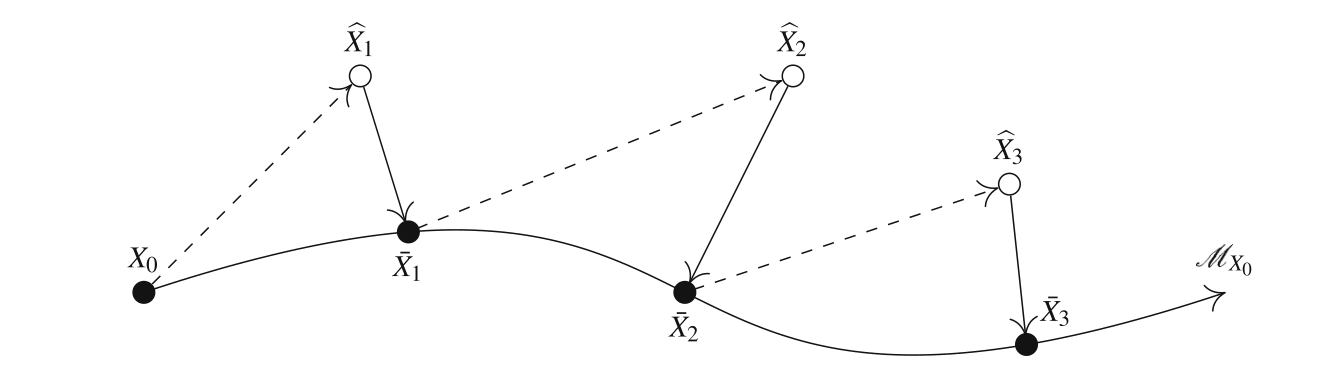
\includegraphics[width=4.95in]{images/project.png}}
	\vspace{.2cm}
	\caption{投射方法}
	\label{fig.5}
\end{figure}

有 $X(t) \in \mathscr M_{X_0} := \{ x\in\R^d : I(x) = I(X_0) \},\quad t\in[0,T],\quad \rm{a.s.}$.



\begin{algorithm}[!htbp]
	\caption{投射方法求解带守恒量的自治随机微分方程}%算法名字
	\LinesNumbered %要求显示行号
	\KwIn{SDE 系统、单步方法的数值格式}%输入参数
	%\KwOut{output result}%输出
	%将 \ito 型随机微分方程处理成 Stratonovich 型随机微分方程\;
	%寻找合适的反对称矩阵 $S,T$,将微分方程处理成 $SG$形式\;
	%构造格式的对称离散梯度 $\overline \nabla I$\;
	%拆分成 $\frac{d(d-1)}{2}$ 个子系统\; 
	\For{\rm{i in \{1,2,…,N\}}}{
		计算单步方法的结果 $\overline X_{t,x}$\;
		计算梯度方向$\Phi \in \R^d$\;
		计算步长$\lambda$\;
		更新守恒解$\widehat X_{t,x} = \overline X_{t,x} + \lambda\Phi$\;
	}
\end{algorithm}


该算法存在两个问题,无法确定投射方向 $\Phi$ 和 $\lambda$ 可能无解. 关于第一个问题,可以用前一个迭代点的 $\overline X$ 的法方向作为投射的梯度方向 $\Phi$,当步长 $h$ 较小且 $\mathscr M_{X_0}$ 较平缓时,该算法的处理是可行的. 但当守恒量流形维度小于 $d-1$ 时,可能无法投射到守恒量所在流形上,导致 $\lambda$ 无解. 

对此,本文提出按照 $L^2$ 距离最短的方式选取投射点. 即如下约束优化问题:
\begin{equation}
	\begin{aligned}
	\begin{aligned}
	&\min _ {\overline X \in \R^d} \frac12 \| \overline X - \widehat X\|_2,\\
	&\qquad \rm{s.t.}\qquad  	I(\overline X) = I(X_0)
	\end{aligned}
	\end{aligned} 
\end{equation}
考虑 SDE 带有 $r$ 个守恒量 $I_1,I_2,\cdots,I_r$,则对应的拉格朗日乘子函数为:
\[
L(x_1,x_2,\cdots ,x_d,\lambda_1,\cdots,\lambda_r) = \frac12 \sum _{i=1}^{d} (x_i-\widehat X_i)^2 + \sum_{i=1}^r \lambda_i( I_i(x) - I_i(\widehat X)). 
\]
分别关于 $d$ 个变量和 $r$ 个乘子参数求导,得 $d+r$ 个方程,导入非线性方程求解器,即可得到 $L^2$ 距离最近意义下的投射点. 非线性方程求解器的迭代初始点设置为 $\widehat X$,能很快收敛到 $\overline X$. 
相对于原方法,改进方法投射点更合理,不需要在法空间中确定具体的投射方向,且算法很容易实现. 


\section{带守恒量问题的稳定解}
本节之前部分讨论的均为保持单一样本轨道的守恒量,现考虑随机系统的稳定解. 对于存在稳定解的带守恒量的自治随机微分方程,不同的初值设置下,守恒量初值是可以不同的,因而对应的稳定解也不唯一. 根据守恒量可以对稳定解进行分类. 

由于稳定解不唯一,仅考虑精度的数值格式很可能无法收敛到相应初值下的稳定解,本文提出使用保守恒量的数值格式可以得到带守恒量的问题的稳定解. 数值实验中,对于一个守恒量为 $\frac12(x_1^2+x_2^2)$ 的随机系统进行数值模型,有如下结果:


\begin{figure}[!htbp]
	\centering 
	\subfigure[$x_1$的稳定解]{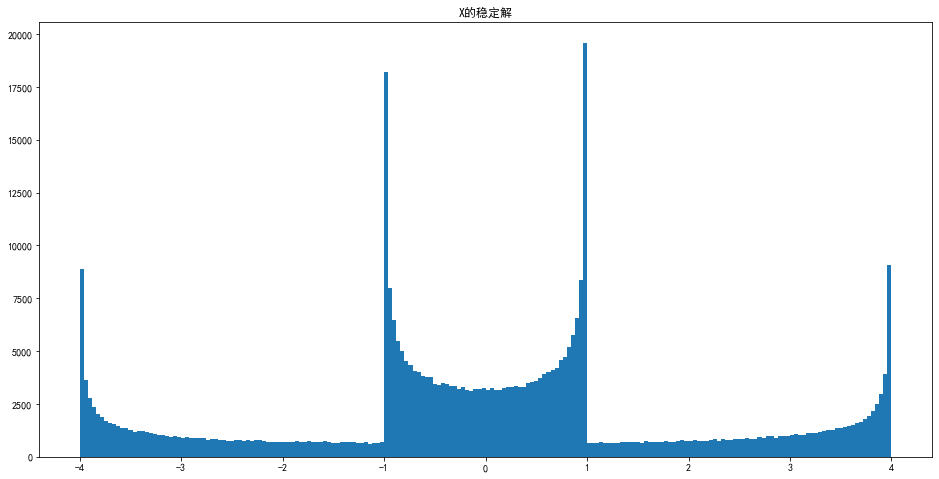
\includegraphics[width=2.95in]{images/5.4/1-x.png}}
	\subfigure[$x_2$的稳定解]{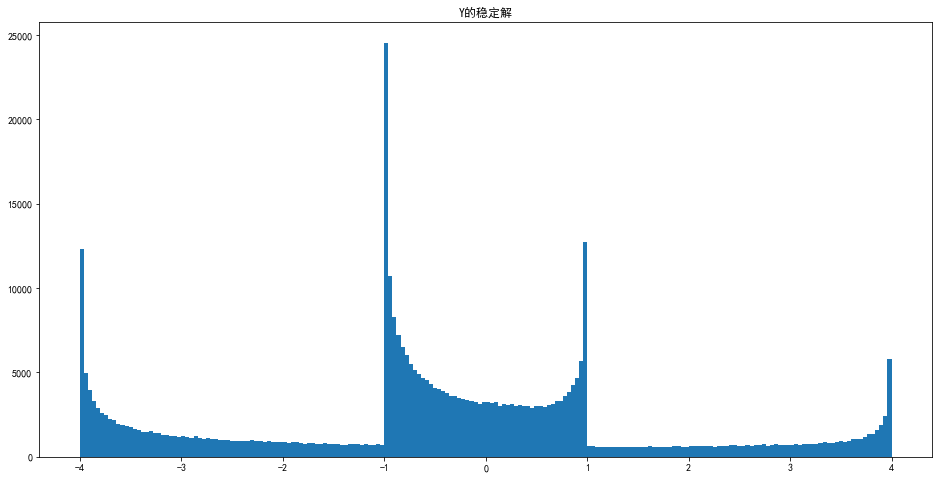
\includegraphics[width=2.95in]{images/5.4/1-y.png}}
	\vspace{.2cm}
	\caption{初值分布为两点分布下的稳定解}
	\label{fig.5.2}
\end{figure}

\begin{figure}[!htbp]
	\centering 
	\subfigure[$x_1$的稳定解]{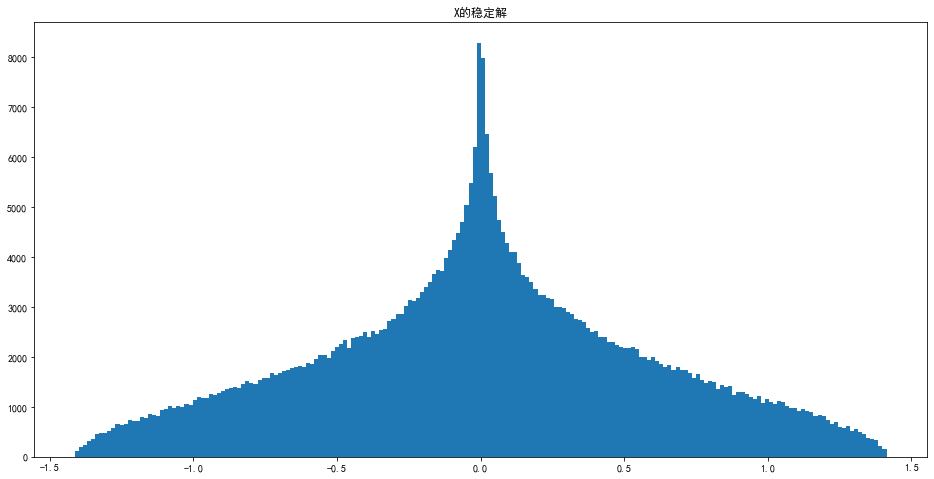
\includegraphics[width=2.95in]{images/5.4/2-x.png}}
	\subfigure[$x_2$的稳定解]{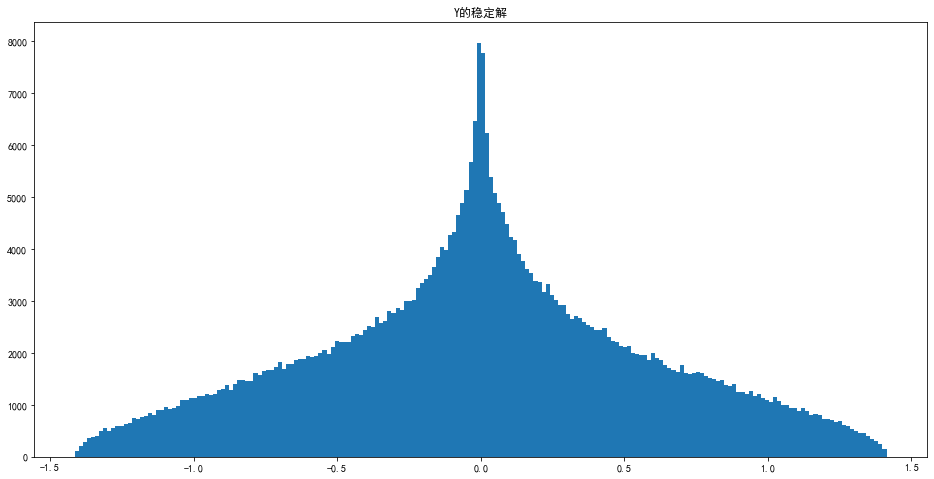
\includegraphics[width=2.95in]{images/5.4/2-y.png}}
	\vspace{.2cm}
	\caption{初值分布为均匀分布的稳定解}
	\label{fig.5.3}
\end{figure}

图\ref{fig.5.2}的初值分布为 $P((x_1,x_2) = (0,1) ) = \frac12$,$P((x_1,x_2) = (0,4) ) = \frac12$. 图\ref{fig.5.2}的初值分布 $x_1=x_2$ 服从分布 $U(0,1]$,考虑的方程均为二维随机 Kubo oscillator 方程. 

本文将带守恒量的自治随机微分方程的稳定解的加速算法总结为:
\begin{algorithm}[!htbp]
	\caption{带守恒量的自治随机微分方程的稳定解的加速算法}%算法名字
	\LinesNumbered %要求显示行号
	\KwIn{SDE 系统,误差界$\varepsilon$,样本轨道数$N$}%输入参数
	%\KwOut{output result}%输出
	$X = \mathcal N(0,1,N),\quad h=0.1,\quad \rm{time} = 0$\;
	\For{\rm{i in \{0,1,2,…,10\}}}{
		h = h / 2 \;
		M = pow(2,i)\;
		\For{\rm{j in \{0,1,2,…,M\}}}{
			time = time + h\;
			newX = scheme(X,h) \# 单步方法  \;
			newX = project(X,$I_1,\cdots,I_r$) \# 投射操作\; 
			\If{$\|\rm{sort(newX)-sort(X)}\| < \varepsilon$}{
				break\;
			}\Else{
				newX = X\;
			}
		}
	}
\end{algorithm}

根据实验,本文推测通过限制守恒量的方式,离散算法的稳定解是收敛的. 




